% Settings for the default beamer theme
\documentclass[english, aspectratio=169]{beamer}
\usepackage[T1]{fontenc}
\usepackage[utf8]{inputenc}
\usepackage{adjustbox}
\usepackage{tabularx}
\usepackage{listings}
\usepackage{graphicx}
\usepackage{array}
\usepackage{babel}
\usepackage[ruled,vlined]{algorithm2e}
\usepackage{blkarray}
\SetAlgorithmName{Algoritmus}{algoritmus}{List of Algorithms}
\setcounter{secnumdepth}{3}
\setcounter{tocdepth}{3}

\makeatletter

\newcommand\makebeamertitle{\frame{\maketitle}}

% (ERT) argument for the TOC
\AtBeginDocument{%
	\let\origtableofcontents=\tableofcontents
	\def\tableofcontents{\@ifnextchar[{\origtableofcontents}{\gobbletableofcontents}}
	\def\gobbletableofcontents#1{\origtableofcontents}
}

% Theme settings
\usetheme{Frankfurt}
\usecolortheme{default}
\usefonttheme[onlymath]{serif}

% Template settings
\setbeamertemplate{navigation symbols}{}
\setbeamertemplate{blocks}[rounded][shadow=false]
\setbeamertemplate{title page}[default][colsep=-4bp, rounded=true, shadow=false]
\makeatother

% Custom color definitions
\definecolor{lightgrey}{gray}{0.95}
\definecolor{DarkerGreen}{RGB}{0,85,0} % Adjust the RGB values as needed

% Use the newly defined color in Beamer theme elements
\setbeamercolor{structure}{fg=DarkerGreen} % Changes basic structural elements to Darker Green
\setbeamercolor{title in head/foot}{bg=DarkerGreen} % Changes the title in header/footer to Darker Green

% Definitions for program code sections
\lstset{
	language=bash,
	basicstyle=\ttfamily\footnotesize, % Monospace font
	backgroundcolor=\color{lightgrey}, % Background color
	frame=single, % Frame around the code
	keywordstyle=\color{black}, % Keywords color
	commentstyle=\color{black}, % Comments color
	stringstyle=\color{red}, % Strings color
	showstringspaces=false, % Do not show spaces in strings
	breaklines=true, % Automatically break long lines
}

\lstset{
	language=python,
	basicstyle=\ttfamily\scriptsize, % Basic font style
	keywordstyle=\bfseries\color{blue}, % Keywords in bold and blue
	stringstyle=\color{red}, % Strings in red
	commentstyle=\color{green!50!black}, % Comments in green
	showstringspaces=false, % Do not show spaces in strings
	numbers=left, % Line numbers on the left
	numberstyle=\tiny\color{gray}, % Line number style
	stepnumber=1, % Line number step
	numbersep=5pt, % Distance of line numbers from code
	frame=single, % Frame around the code
	rulecolor=\color{black}, % Frame color
	tabsize=2, % Tab size
	breaklines=true, % Automatic line breaking
	breakatwhitespace=false, % Break lines at whitespace
	captionpos=b, % Caption position
	escapeinside={\%*}{*)}, % Escape to LaTeX
	morekeywords={self}, % Additional keywords
}

\begin{document}
	% Title page
	\section{Bevezetés}
	\title[]{Adatbányászat a Gyakorlatban}
	\subtitle{2. Gyakorlat: Dash alapok}
	\author[Kuknyó Dániel]{Kuknyó Dániel\\Budapesti Gazdasági Egyetem}
	\date{2024/25\\1.félév}
	\makebeamertitle
	
	% Table of contents slide
	\begin{frame}
		\tableofcontents{}
	\end{frame}
	
	% Table of contents of the current section
	\begin{frame}
		\tableofcontents[currentsection]
	\end{frame}
	
	\begin{frame}[fragile]{Órai környezet telepítése}
		\begin{enumerate}
			\item Új Anaconda környezet létrehozása \texttt{dash} néven:
			\begin{lstlisting}
$ conda create --name dash python=3.12
			\end{lstlisting}
			\item Környezet aktiválása:
			\begin{lstlisting}
$ conda activate dash
			\end{lstlisting}
			\item Órai tárhely klónozása:
			\begin{lstlisting}
$ git clone https://github.com/basictask/Adatbanyaszat.git
			\end{lstlisting}
			\item Függőségek telepítése:
			\begin{lstlisting}
$ cd Adatbanyaszat
$ pip install -r requirements.txt
			\end{lstlisting}
		\end{enumerate}
	\end{frame}
	
	\begin{frame}{A Dash keretrendszer}
		A Dash keretrendszer segítségével lehetséges interaktív, dinamikus adatalapú műszerfalakat és alkalmazásokat készíteni színtisztán Python nyelvben.\par\smallskip
		A Dash a ~\textbf{Flask} mikrokeretrendszert használja backend szerverként, \textbf{Plotly} segítségével jelenítui meg a diagramokat és \textbf{React} komponenseket használ a felhasználói interakció kezelésére.
		\vspace{0.4cm}
		\begin{center}
			\begin{tabular}{c c c c c c c}
				\adjustbox{valign=c}{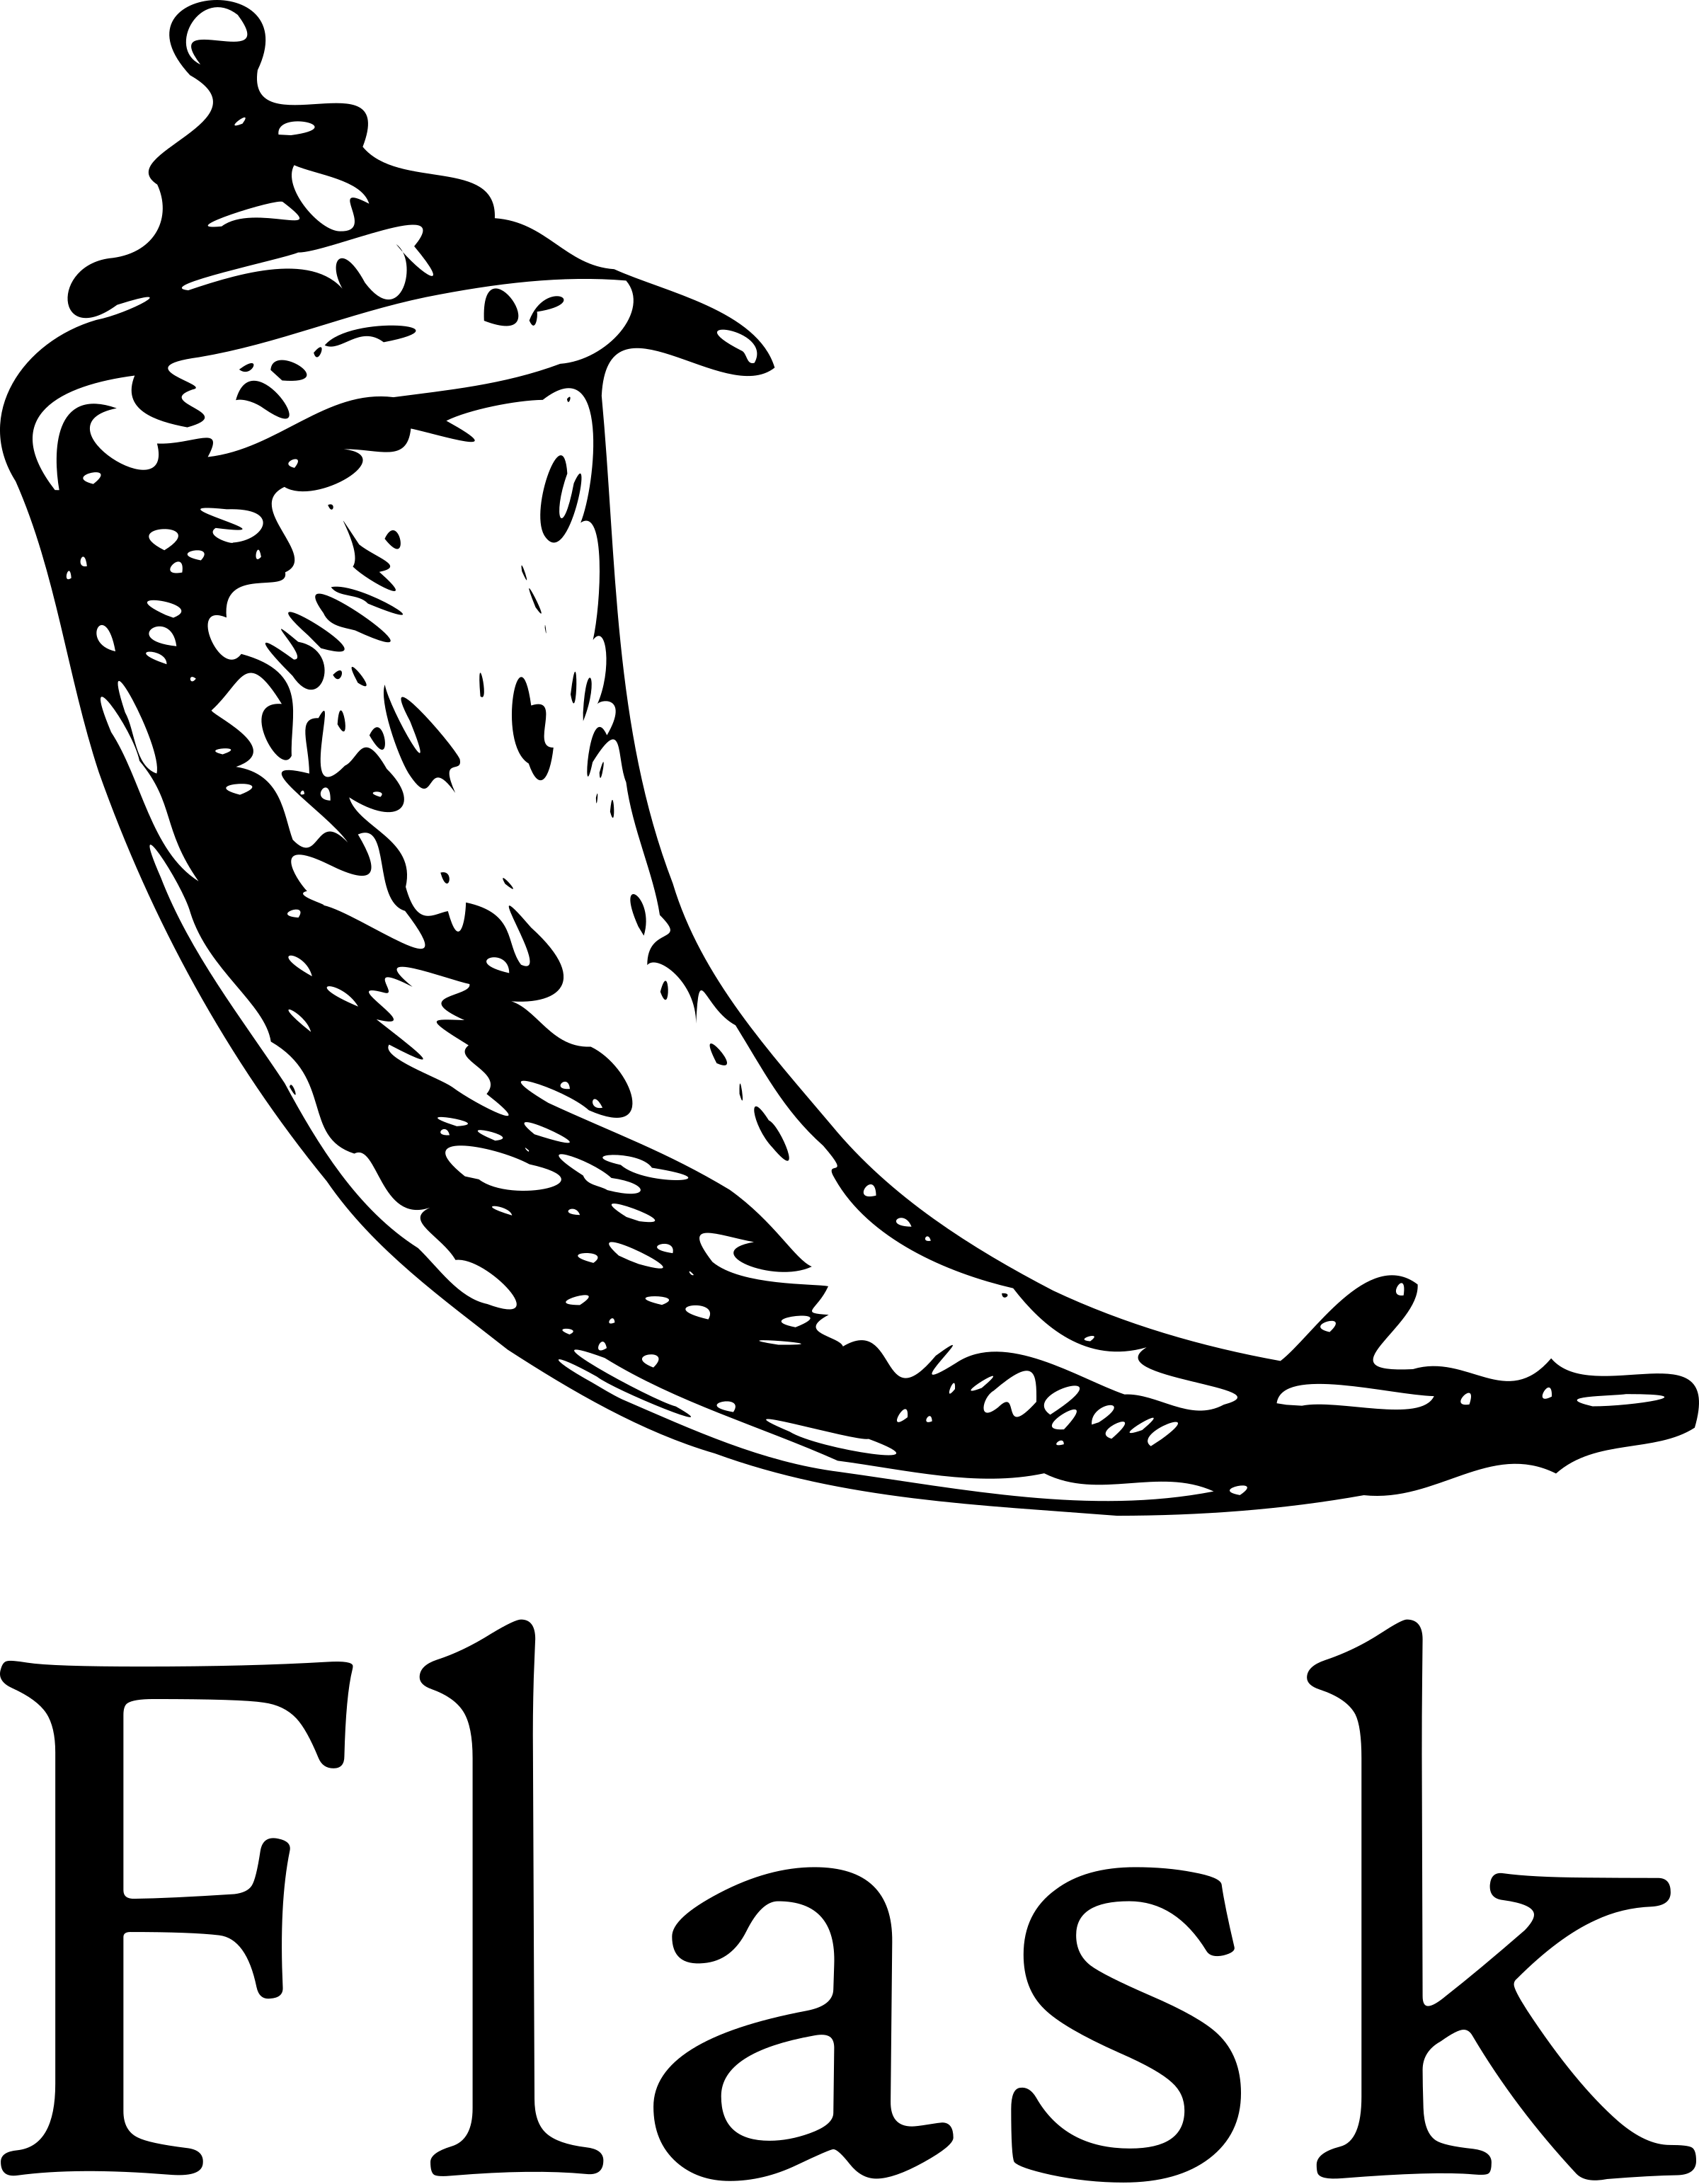
\includegraphics[height=1.5cm, keepaspectratio]{images/dash_1.png}} &
				\adjustbox{valign=c}{+} &
				\adjustbox{valign=c}{
\includegraphics[height=1.5cm, keepaspectratio]{images/dash_2.png}} &
				\adjustbox{valign=c}{+} &
				\adjustbox{valign=c}{
\includegraphics[height=1.5cm, keepaspectratio]{images/dash_3.png}} &
				\adjustbox{valign=c}{=} &
				\adjustbox{valign=c}{
\includegraphics[height=1cm, keepaspectratio]{images/dash_4.png}} \\
			\end{tabular}
		\end{center}
	\end{frame}
	
	\begin{frame}[fragile]{A Dash könyvtár komponensei}
		\only<1>{
			\begin{block}{Dash}
				Ez a fő csomag, amely bármely alkalmazás gerincét biztosítja a \texttt{dash.Dash} objektumon keresztül.\par\smallskip
				Emellett néhány más eszközt is biztosít az interaktivitás és kivételek kezeléséhez, amelyekről később fogunk beszélni, amikor építjük az alkalmazásunkat.
		\end{block}}
		\only<2>{
			\begin{block}{Dash Core Components}
				Egy csomag, amely interaktív komponensek készletét biztosítja, amelyeket a felhasználók manipulálhatnak.\par\smallskip
				Legördülő menük, dátumválasztók, csúszkák és sok más komponens is megtalálható ebben a csomagban.
		\end{block}}
		\only<3>{
			\begin{block}{Dash HTML Components}
				Ez a csomag az összes elérhető HTML címkét Python osztályként biztosítja. Egyszerűen átalakítja a Pythont HTML-re.\par\smallskip
				Például, Pythonban a \texttt{dash\_html\_components.H1('Hello, World')} kód átalakul \texttt{<h1>Hello, World</h1>} HTML kóddá.
		\end{block}}
		\only<4>{
			\begin{block}{Dash Bootstrap Components}
				Ez egy harmadik féltől származó csomag, amely Bootstrap funkcionalitást ad a Dash-hez. Ez a csomag és annak komponensei számos elrendezéssel és vizuális jelekkel kapcsolatos lehetőséget kezelnek.\par\smallskip
				Az elemek egymás mellé vagy egymás fölé helyezése, méretük meghatározása a böngésző képernyőmérete alapján, valamint kódolt színek készletének biztosítása a jobb kommunikáció érdekében a felhasználókkal.
		\end{block}}
	\end{frame}
	
	\begin{frame}[fragile]{Egy Dash alkalmazás struktúrája}
		\begin{columns}
			\begin{column}{.5\textwidth}
				\begin{itemize}
					\item Importálások:
					\begin{lstlisting}
import dash
import dash_html_components as html
import dash_core_components as dcc
					\end{lstlisting}
					\item Elrendezés:
					\begin{lstlisting}
app.layout = html.Div([
	dcc.Dropdown()
	dcc.Graph()
	...	
])
					\end{lstlisting}
				\end{itemize}
			\end{column}
			\begin{column}{.5\textwidth}
				\begin{itemize}
					\item Visszahívási függvények:
					\begin{lstlisting}
@app.callback()
...
@app.callback()
...
					\end{lstlisting}
					\item Alkalmazás példányosítása:
					\begin{lstlisting}
app = dash.Dash(__name__)
					\end{lstlisting}
					\item Alkalmazás futtatása:
					\begin{lstlisting}
if __name__ == '__main__':
	app.run_server()
					\end{lstlisting}
				\end{itemize}
			\end{column}
		\end{columns}
	\end{frame}
	
	\section{Komponensek}
	
	\begin{frame}
		\tableofcontents[currentsection]
	\end{frame}
	
	\begin{frame}[fragile]{Egy kezdeti alkalmazás}
		\begin{enumerate}
			\item Egy új, \texttt{app.py} fájlban a következő csomagok importálásával:
			\begin{lstlisting}
import dash
import dash_core_components as dcc
			\end{lstlisting}
			\item Alkalmazás példányosítása:
			\begin{lstlisting}
app = dash.Dash(__name__)
			\end{lstlisting}
			\item Alkalmazás elrendezésének létrehozása:
			\begin{lstlisting}
app.layout = html.Div([
	html.H1('Hello, World!')
])
			\end{lstlisting}
			\item Futtatás:
			\begin{lstlisting}
if __name__ == '__main__':
	app.run_server(debug=True)
			\end{lstlisting}
		\end{enumerate}
	\end{frame}
	
	\begin{frame}[fragile]{Az alkalmazás futtatása (\texttt{app\_v1\_1.py})}
		\begin{columns}
			\begin{column}{.5\textwidth}
				A Python értelmező segítségével a megfelelő könyvtárban állva az \texttt{app\_v1\_1.py} fájl futtatásával az eredmény a következő:
				\begin{lstlisting}[language=python]
(dash) daniel@neptune:~/Documents/BGE/Adatbanyaszat/2_dash/code$ python app_v1_1.py
Dash is running on http://127.0.0.1:8050/

* Serving Flask app 'app_v1_1'
* Debug mode: on
				\end{lstlisting}
			\end{column}
			\begin{column}{.5\textwidth}
				A böngészőben a \texttt{127.0.0.1:8050} címre navigálva a következő eredmény látható:
				\begin{center}
					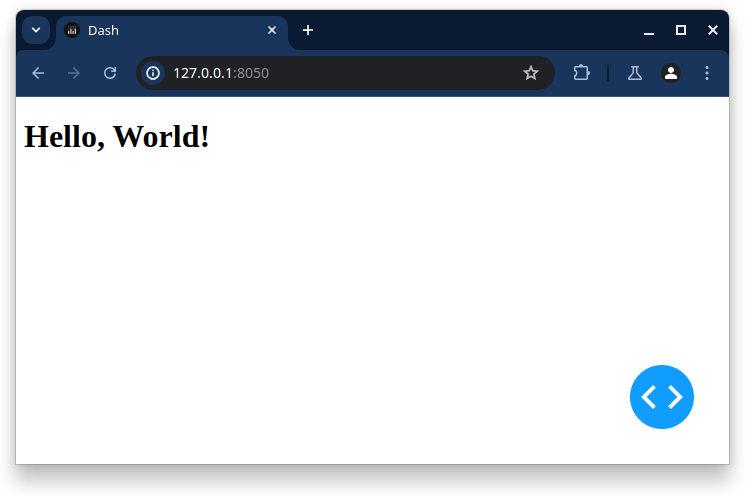
\includegraphics[width=5cm, height=5cm, keepaspectratio]{images/dash_5.png}
				\end{center}
			\end{column}
		\end{columns}
	\end{frame}
	
	\begin{frame}[fragile]{Komponensek hozzáadása az alkalmazáshoz}
		Komponensek hozzáadása az alkalmazás elrendezésének szerkesztésével érhető el (\texttt{app.layout}). Ez meglehetősen egyszerű, csak a legfelső szintű \texttt{html.Div} komponens \texttt{children} attribútumához kell hozzáfűzni a megfelelő elemeket.\par\smallskip
		\begin{lstlisting}[language=python]
html.Div(children=[component_1, component_2, component_3, ...])
		\end{lstlisting}
		\par\smallskip
		\begin{block}{\texttt{Div}}
			A \textbf{\texttt{Div}} a HTML-ben egy blokk szintű elem, amely képes egy dokumentum különböző komponenseit csoportosítani. A \texttt{Div} nem rendelkezik semmilyen alapértelmezett stílussal vagy viselkedéssel.
		\end{block}
	\end{frame}
	
	\begin{frame}[fragile]{HTML komponensek hozzáadása}
		\begin{block}{\texttt{children}}
			Ez az első, és a fő konténere a komponenseknek. Paraméterül kaphatja elemek listáját vagy egyetlen elemet is.
		\end{block}
		\begin{block}{\texttt{className}}
			Ez megegyezik a HTML \texttt{class} attribútumával.
		\end{block}
		\begin{block}{\texttt{id}}
			A komponens azonosítója. Az interaktivitás megvalósításában van kulcsfontosságú szerepe
		\end{block}
		\begin{block}{\texttt{style}}
			Ez megfelel az azonos nevű HTML attribútumnak azzal a különbséggel, hogy camelCase stílust használ a változók elnevezésére.
		\end{block}
	\end{frame}
	
	\begin{frame}{A Dash alkalmazás HTML komponensekkel (\texttt{app\_v1\_2.py})}
		\begin{center}
			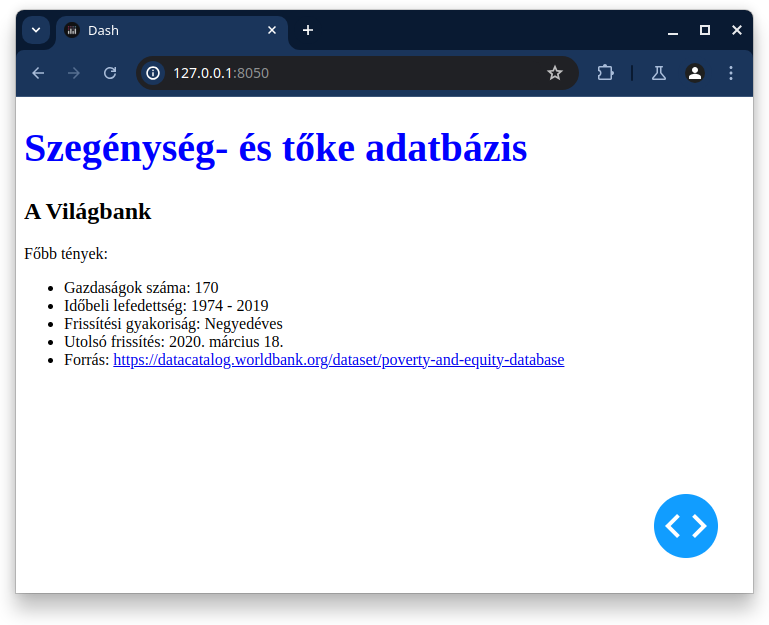
\includegraphics[width=10cm, height=6cm, keepaspectratio]{images/dash_6.png}
		\end{center}
	\end{frame}
	
	\section{Elrendezés}
	
	\begin{frame}{}
		\tableofcontents[currentsection]
	\end{frame}
	
	\begin{frame}[fragile]{Témák}
		Egy Dash alkalmazás témájának megváltoztatása rendkívül egyszerű: a Dash objektum létrehozásakor kell egy új téma argumentumot bevinni a konstruktor függvénybe.\par\medskip
		\begin{lstlisting}[language=python]
import dash_bootstrap_components as dbc
...
app = dash.Dash(__name__, external_stylesheets=[dbc.themes.BOOTSTRAP])
...
		\end{lstlisting}
	\end{frame}
	
	\begin{frame}{Témák az előző alkalmazásban (\texttt{app\_v1\_3.py})}
		\begin{columns}
			\begin{column}{.5\textwidth}
				\begin{center}
					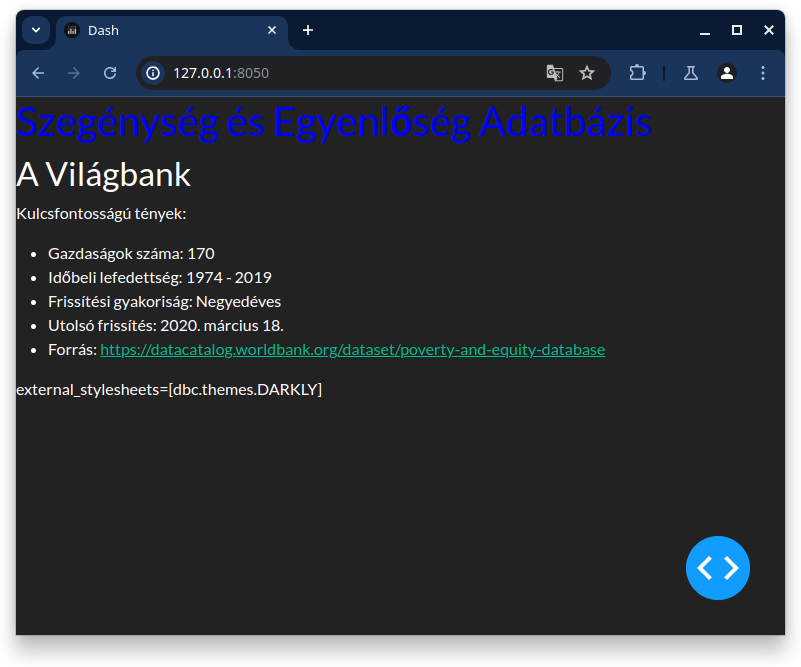
\includegraphics[width=7cm, height=7cm, keepaspectratio]{images/dash_7.png}
				\end{center}
			\end{column}
			\begin{column}{.5\textwidth}
				\begin{center}
					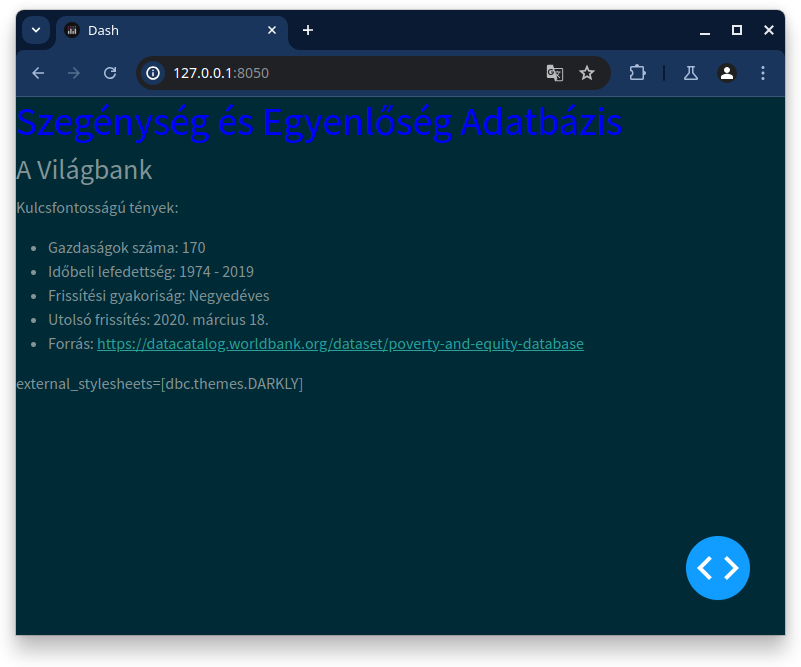
\includegraphics[width=7cm, height=7cm, keepaspectratio]{images/dash_8.png}
				\end{center}
			\end{column}
		\end{columns}
	\end{frame}
	
	\begin{frame}[fragile]{A rács rendszer}
		\begin{columns}
			\begin{column}{.5\textwidth}
				A Bootstrap segítségével lehetséges oszlopokat definiálni, ami egy független képernyőként viselkedik, egymás fölött megjelenítve az elemeket.\par\medskip
				A rács rendszer 12 oszlopra bontja a képernyőt, és egy komponens szélessége oszlopok számában adható meg. 
			\end{column}
			\begin{column}{.6\textwidth}
				\begin{center}
					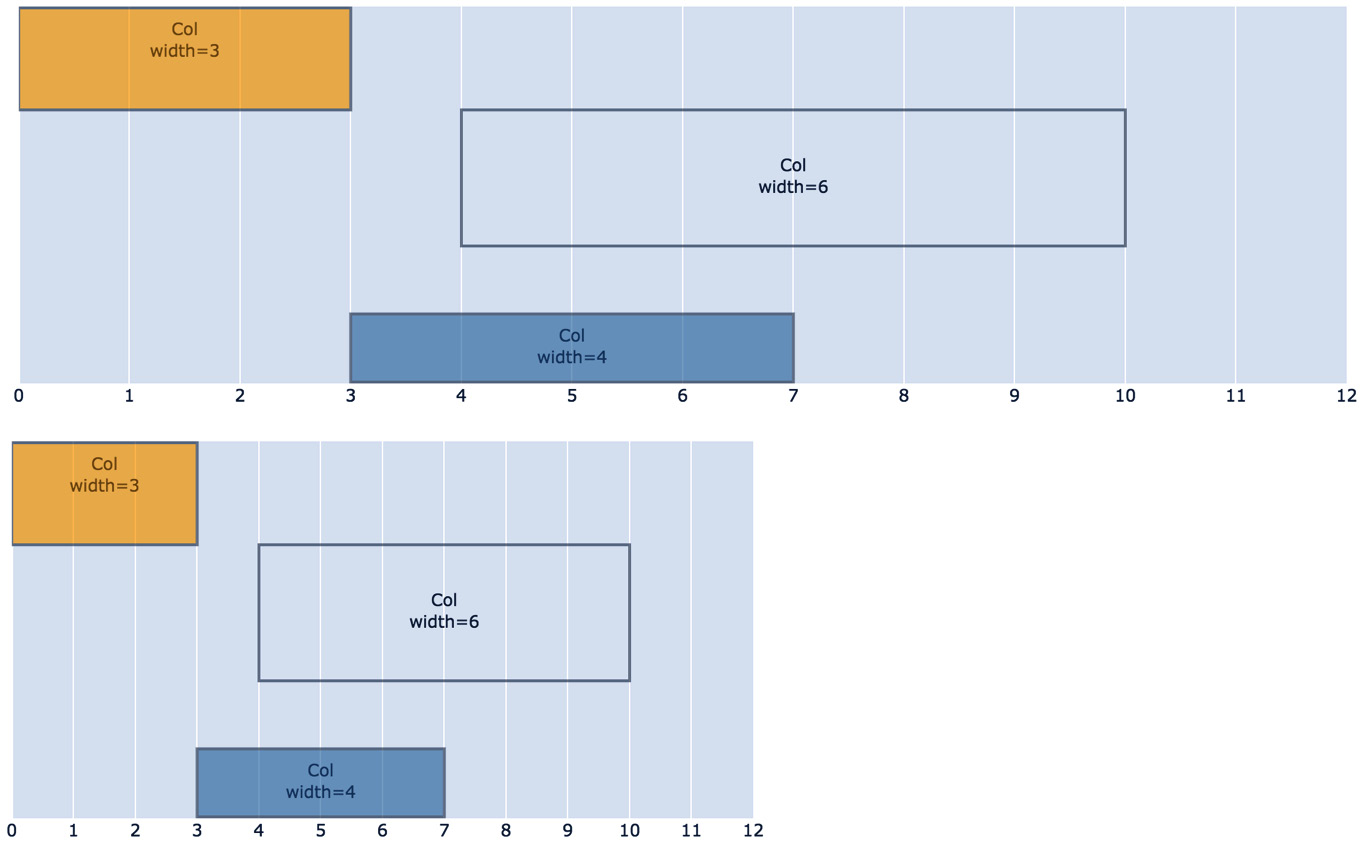
\includegraphics[width=7cm, keepaspectratio]{images/dash_9.png}
				\end{center}
			\end{column}
		\end{columns}
		\vspace{0.2cm}
		\begin{center}
			\begin{lstlisting}[language=python]
import dash_boostrap_components as dbc
dbc.Col(children=[child1, child2, ...])
			\end{lstlisting}
		\end{center}
	\end{frame}
	
	\begin{frame}[fragile]{Rácsok dinamikus képernyő méreten}
		\begin{columns}
			\begin{column}{.4\textwidth}
				Vannak olyan esetek, amikor nem kívánatos az elemek méretezése a képernyővel együtt. Amikor a képernyő kisebb lesz, némelyik komponenseknek jó, ha kiterjednek méretükben.\par\smallskip
				Öt különböző méretet lehet definiálni: \texttt{xs} (extra-small), \texttt{md} (medium), \texttt{lg} (large), \texttt{xl} (extra-large).
			\end{column}
			\begin{column}{.6\textwidth}
				\begin{center}
					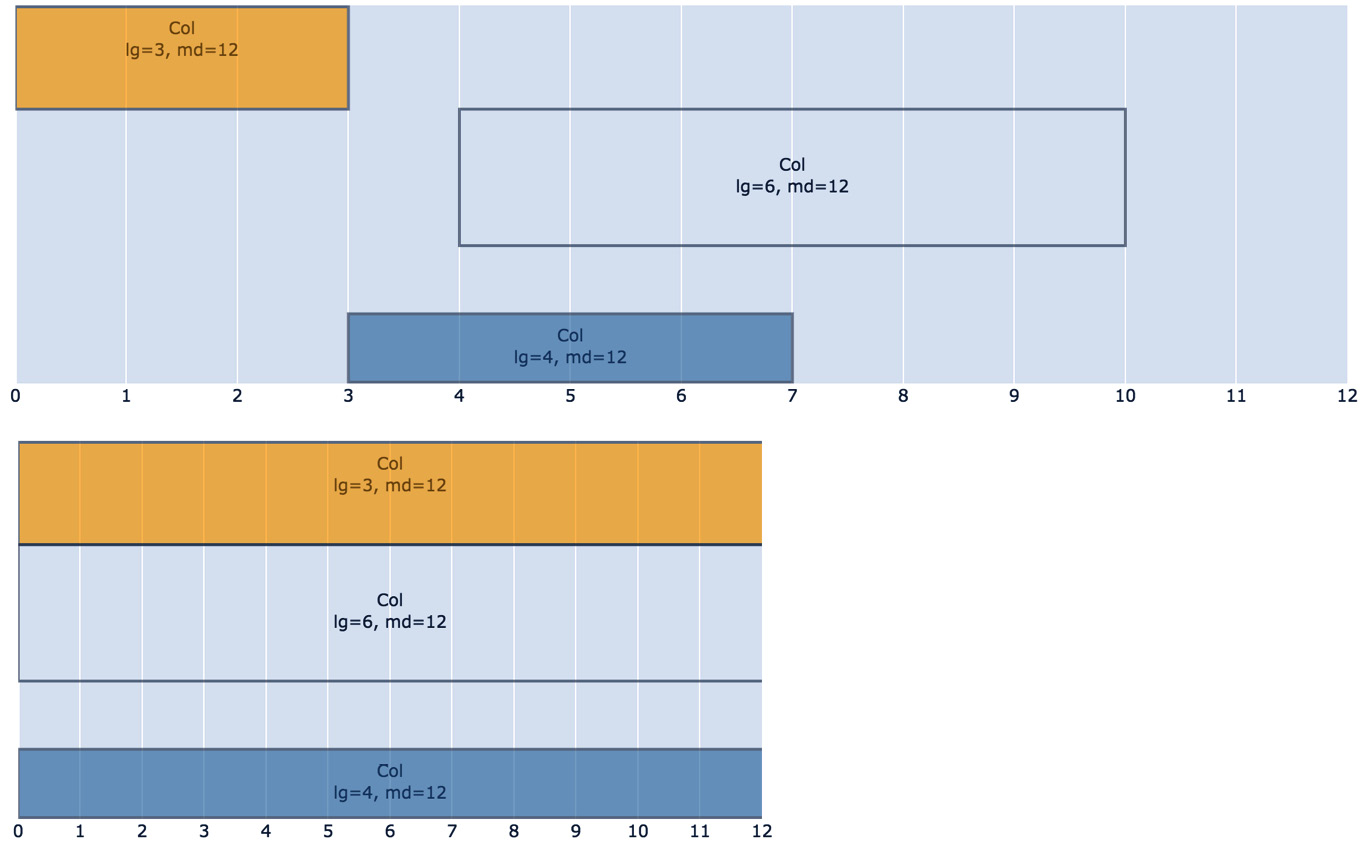
\includegraphics[width=7cm, keepaspectratio]{images/dash_10.png}
				\end{center}
			\end{column}
		\end{columns}
		\vspace{0.2cm}
		\begin{center}
			\begin{lstlisting}[language=python]
import dash_boostrap_components as dbc
dbc.Col(children=[child1, child2, ...], lg=6, md=12)
			\end{lstlisting}
		\end{center}
	\end{frame}
	
	\begin{frame}[fragile]{Bootstrap komponensek hozzáadása az alkalmazáshoz (\texttt{app\_v1\_4.py})}
		\begin{columns}
			\begin{column}{.5\textwidth}
				Az alkalmazás következő verziójában két új komponens kerül hozzáadásra, a \texttt{Tabs} és \texttt{Tab}. Ezek szorosan kapcsolódnak egymáshoz. A \texttt{Tabs} a \texttt{Tab} konténere.\par\smallskip
				Ennek eredménye egy informatívabb és jobban elrendezett alkalmazás. 
			\end{column}
			\begin{column}{.5\textwidth}
				\begin{center}
					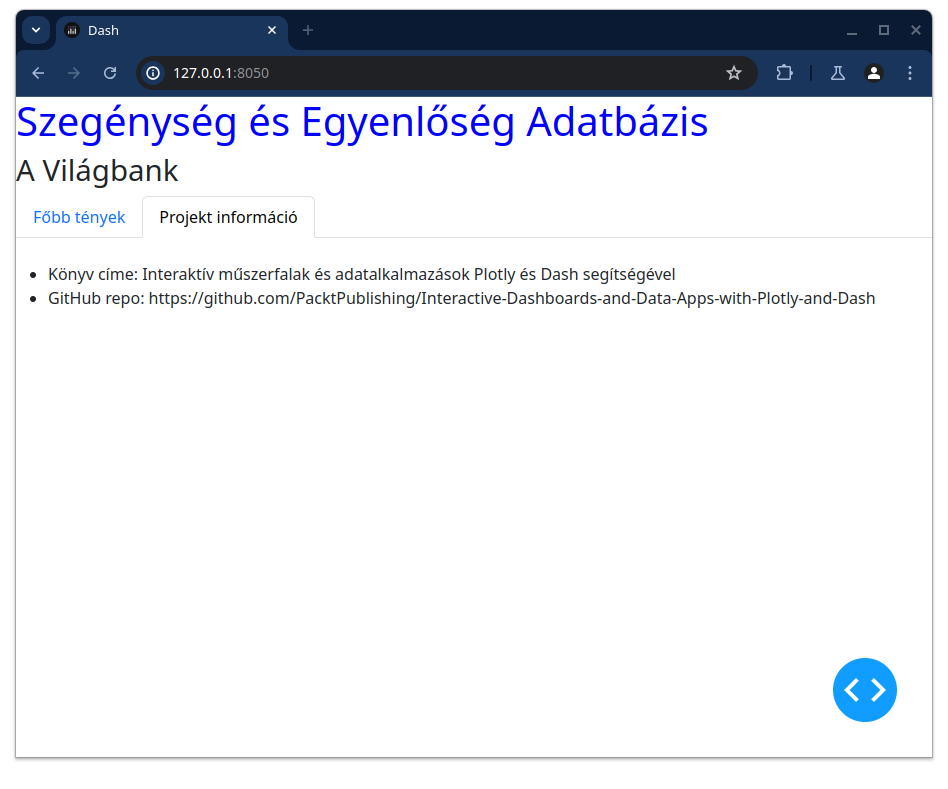
\includegraphics[width=6cm, keepaspectratio]{images/dash_11.png}
				\end{center}
			\end{column}
		\end{columns}
	\end{frame}
	
	\begin{frame}[fragile]{Dash alkalmazások Jupyter Notebookban}
		Kevés programkód változtatással az alkalmazás Jupyter Notebook környezetben is futtathatóvá válik. Ezt a \texttt{jupyter\_dash} csomag teszi lehetővé.\par\smallskip
		A használatához a Dash helyett a JupyterDash csomagot kell importálni, és ennek mentén kell példányosítani az alkalmazást:
		\begin{lstlisting}[language=python]
from jupyter_dash import JupyterDash
app = JupyterDash(__name__)
		\end{lstlisting}
		A JupyterDash három módot biztosít az alkalmazás futtatására:
		\begin{itemize}
			\item \texttt{external}: Külön böngésző ablakban
			\item \texttt{inline}: A kód output helyen a notebookban
			\item \texttt{jupyterlab}: Külön böngészőfülben (csak JupyterLab szerveren)
		\end{itemize}
	\end{frame}
	
	\section{Struktúra}
	
	\begin{frame}
		\tableofcontents[currentsection]
	\end{frame}
	
	\begin{frame}[fragile]{Komponensek \texttt{id} paramétere}
		\begin{columns}
			\begin{column}{.5\textwidth}
				Az \texttt{id} paraméter elengedhetetlen a Dash alkalmazások interaktivitásához.\par\smallskip
				Ez egy, a komponensekhez rendelt egyedi azonosító, amelynek segítségével az alkalmazás megkülönbözteti és kezeli a különböző vezérlőelemeket, például grafikonokat vagy szövegdobozokat.
			\end{column}
			\begin{column}{.5\textwidth}
				\begin{center}
					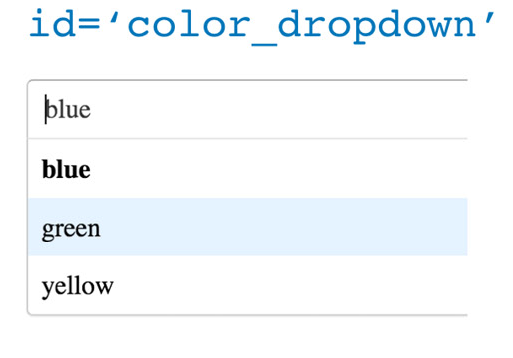
\includegraphics[width=4cm, height=7cm, keepaspectratio]{images/dash_12.png}
				\end{center}
			\end{column}
		\end{columns}
		\medskip
		\begin{lstlisting}
app.layout = html.Div([
	dcc.Dropdown(
		id='color_dropdown',
		options=[{'label': x, 'value': x} for x in ['blue', 'green', 'yellow']]
	)
])				
		\end{lstlisting}
	\end{frame}
	
	\begin{frame}{Callback függvények}
		\begin{columns}
			\begin{column}{.5\textwidth}
				A callback egy Dash alkalmazásban egy olyan függvény, amely akkor hívódik meg, amikor egy adott esemény bekövetkezik, például egy felhasználói interakció.\par\smallskip
				Így dinamikusan frissíthetők az alkalmazás komponensei. A következők szükségesek egy callback függvényhez:
				\begin{itemize}
					\item \texttt{Output}: Az a komponens attribútum, amelyik meg fog változni a függvény hatására. 
					\item \texttt{Input}: Az az alkalmazás elem vagy esemény, amelyik elindítja a függvényt.
					\item A függvény fejléc és definíció. 
				\end{itemize}
			\end{column}
			\begin{column}{.5\textwidth}
				\begin{center}
					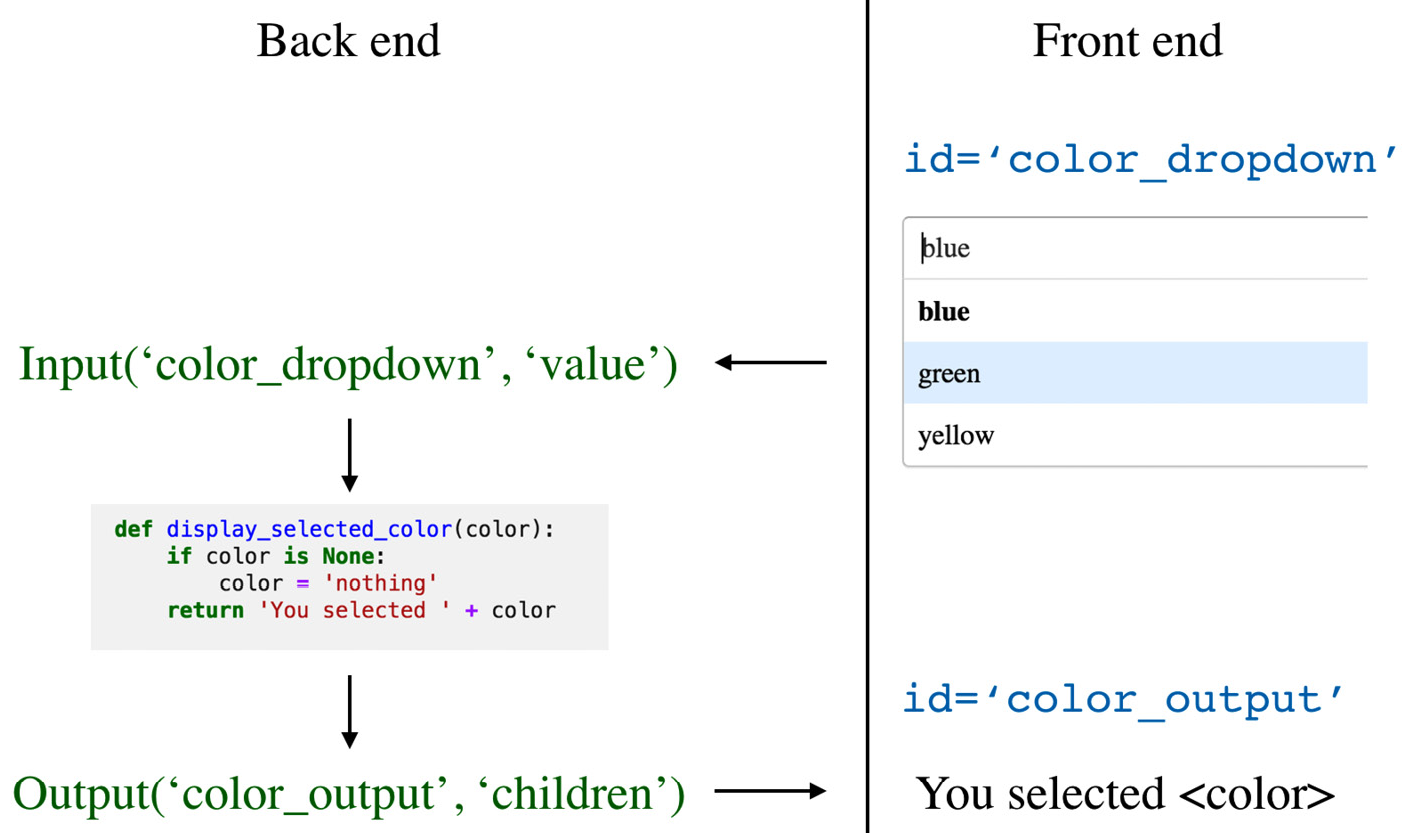
\includegraphics[width=7cm, height=7cm, keepaspectratio]{images/dash_13.png}
				\end{center}
			\end{column}
		\end{columns}
	\end{frame}
	
	\begin{frame}[fragile]{Callback függvény implementálása}
		\begin{columns}
			\begin{column}{.5\textwidth}
				A callback működés egy dekorátor segítségével valósítható meg a függvény fejléce fölött. Itt definiálni kell az \texttt{Input} és \texttt{Output} komponenseket, ilyen sorrendben.\par\smallskip
				Egy callback függvénynek több inputja és outputja lehet.
			\end{column}
			\begin{column}{.5\textwidth}
				\begin{lstlisting}[language=python]
@app.callback(
	Output('color_output', 'children'),
	Input('color_dropdown', 'value')
)
def display_selected_color(color):
	if color is None:	
		color = 'nothing'
		return 'You selected ' + color
				\end{lstlisting}
			\end{column}
		\end{columns}
	\end{frame}
	
	\begin{frame}[fragile]{Callback függvény implementálása az alkalmazásba (\texttt{app\_v1\_5.py})}
		\begin{columns}
			\begin{column}{.5\textwidth}
				Egy callback implementálásának lépései:
				\begin{enumerate}
					\item Új lenyíló lista létrehozása egy adathalmazban megtalálható országok segítségével
					\item Egy új callback függvény létrehozása amely megkapja a választott országot, leszűri az adathalmazt majd megtalálja az ország népességi adatait (az összes forrásfájl a \texttt{data} mappában található). 
					\item Egy riport készítése a megtalált adatokról. 
				\end{enumerate}
			\end{column}
			\begin{column}{.5\textwidth}
				\begin{center}
					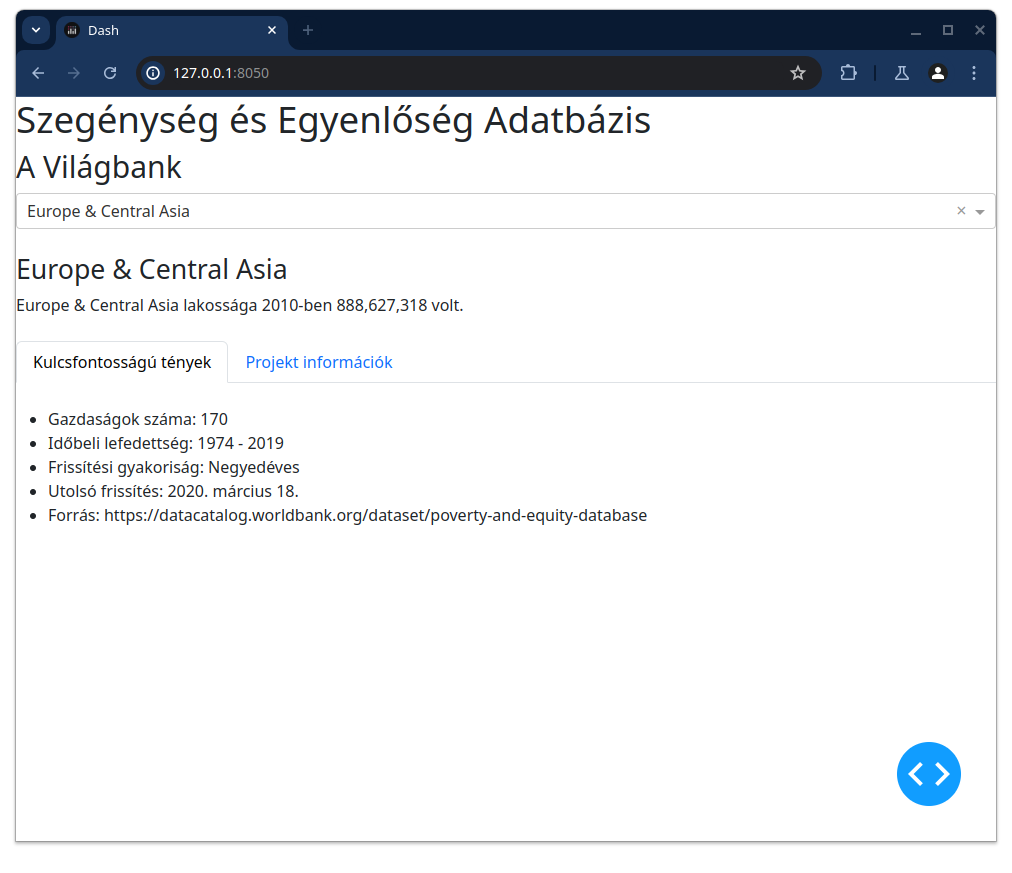
\includegraphics[width=7cm, height=7cm, keepaspectratio]{images/dash_14.png}
				\end{center}
			\end{column}
		\end{columns}
	\end{frame}
	
	\begin{frame}{Callback függvények tulajdonságai}
		\begin{columns}
			\begin{column}{.5\textwidth}
				\begin{itemize}
					\item A visszatérés előtt szinte bármilyen műveletet elvégezhetnek, mint pl. egy gépi tanulás modell tanítása
					\item A callback függvények harmadik attribútuma a (\texttt{State}). Az állapottal definiált objektum attribútumok nem indítják el a callback függvényt, de a futás során a függvény hozzáfér az értékükhöz.
					\item A callback dekorátor definíciós sorrendje: \texttt{[Output, Input, State]}.
					\item Az input és állapot sorrend a callback dekorátorban meg kell feleljen a paraméterek sorrendjének.. 
				\end{itemize}
			\end{column}
			\begin{column}{.5\textwidth}
				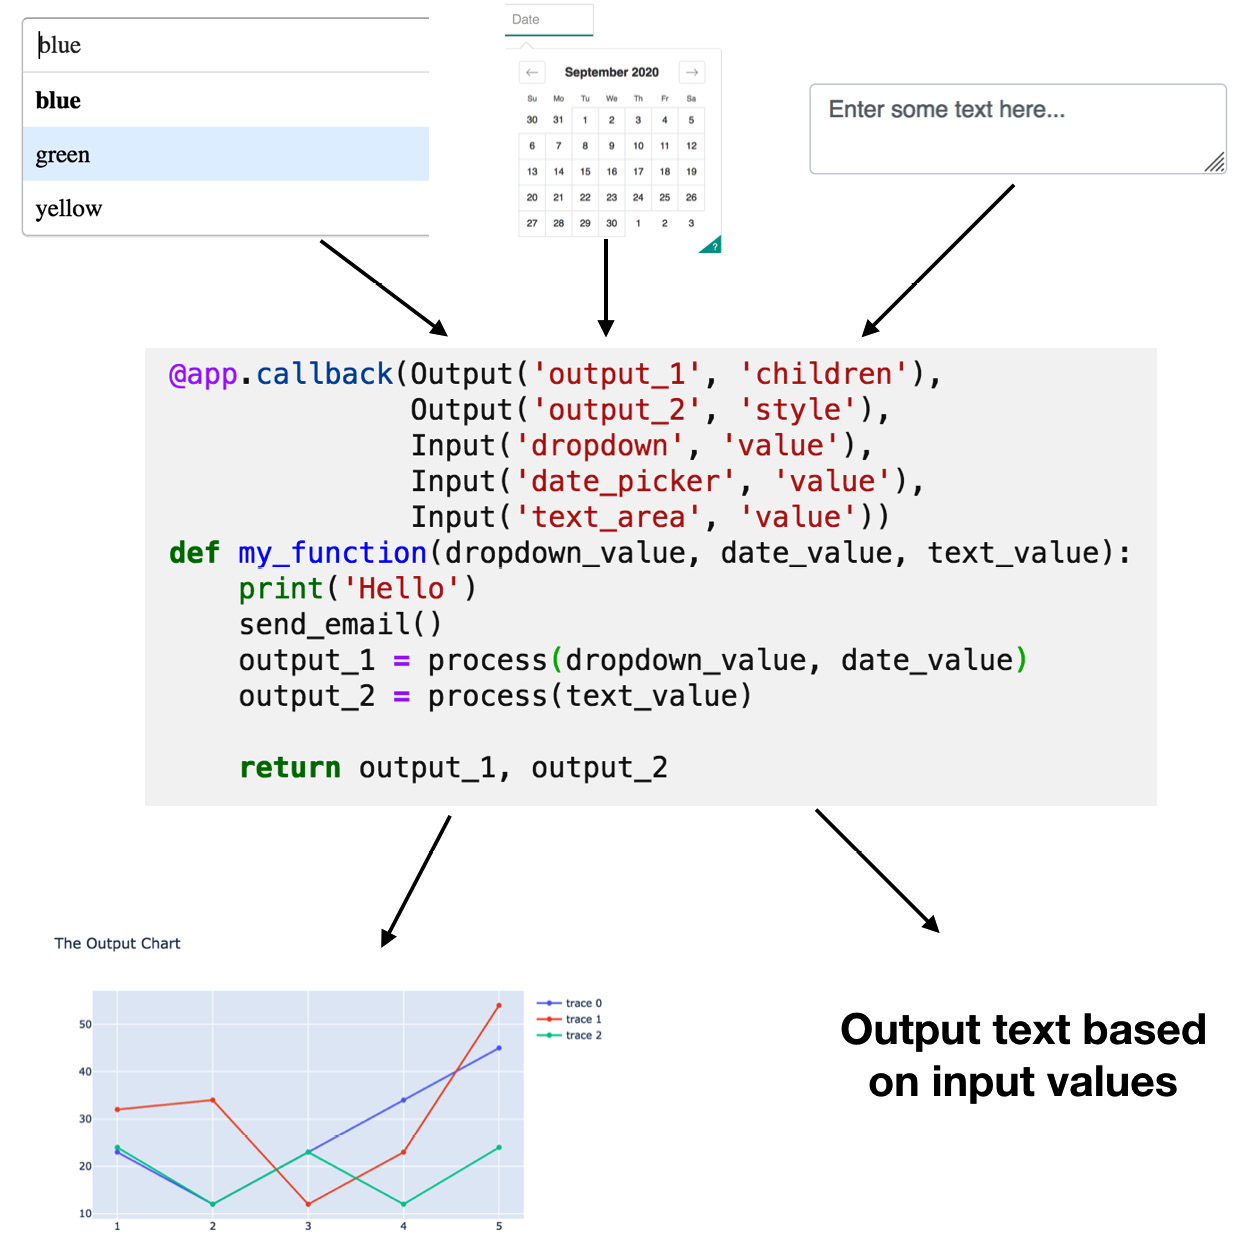
\includegraphics[height=7cm, width=7cm, keepaspectratio]{images/dash_15.png}
			\end{column}
		\end{columns}
	\end{frame}
\end{document}